% Created by tikzDevice version 0.12.3.1 on 2023-04-20 20:37:27
% !TEX encoding = UTF-8 Unicode
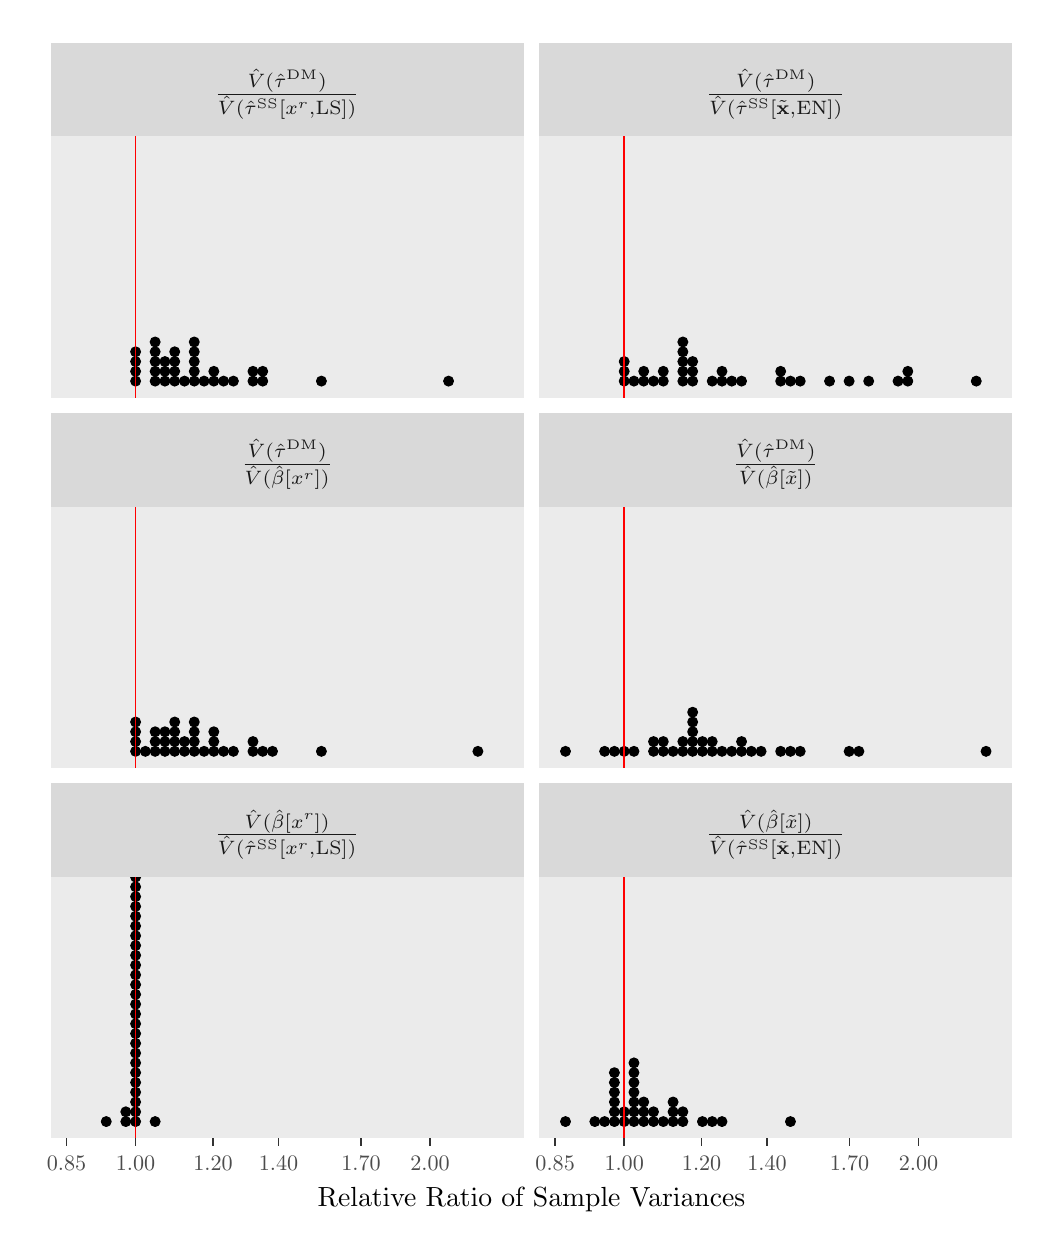
\begin{tikzpicture}[x=1pt,y=1pt]
\definecolor{fillColor}{RGB}{255,255,255}
\path[use as bounding box,fill=fillColor,fill opacity=0.00] (0,0) rectangle (361.35,433.62);
\begin{scope}
\path[clip] (  0.00,  0.00) rectangle (361.35,433.62);
\definecolor{drawColor}{RGB}{255,255,255}
\definecolor{fillColor}{RGB}{255,255,255}

\path[draw=drawColor,line width= 0.6pt,line join=round,line cap=round,fill=fillColor] (  0.00,  0.00) rectangle (361.35,433.62);
\end{scope}
\begin{scope}
\path[clip] (  8.25,299.84) rectangle (179.30,394.32);
\definecolor{fillColor}{gray}{0.92}

\path[fill=fillColor] (  8.25,299.84) rectangle (179.30,394.32);
\definecolor{drawColor}{RGB}{0,0,0}
\definecolor{fillColor}{RGB}{0,0,0}

\path[draw=drawColor,line width= 0.4pt,line join=round,fill=fillColor] ( 39.00,305.90) circle (  1.77);

\path[draw=drawColor,line width= 0.4pt,line join=round,fill=fillColor] ( 39.00,309.43) circle (  1.77);

\path[draw=drawColor,line width= 0.4pt,line join=round,fill=fillColor] ( 39.00,312.97) circle (  1.77);

\path[draw=drawColor,line width= 0.4pt,line join=round,fill=fillColor] ( 39.00,316.50) circle (  1.77);

\path[draw=drawColor,line width= 0.4pt,line join=round,fill=fillColor] ( 46.06,305.90) circle (  1.77);

\path[draw=drawColor,line width= 0.4pt,line join=round,fill=fillColor] ( 46.06,309.43) circle (  1.77);

\path[draw=drawColor,line width= 0.4pt,line join=round,fill=fillColor] ( 46.06,312.97) circle (  1.77);

\path[draw=drawColor,line width= 0.4pt,line join=round,fill=fillColor] ( 46.06,316.50) circle (  1.77);

\path[draw=drawColor,line width= 0.4pt,line join=round,fill=fillColor] ( 46.06,320.04) circle (  1.77);

\path[draw=drawColor,line width= 0.4pt,line join=round,fill=fillColor] ( 49.60,305.90) circle (  1.77);

\path[draw=drawColor,line width= 0.4pt,line join=round,fill=fillColor] ( 49.60,309.43) circle (  1.77);

\path[draw=drawColor,line width= 0.4pt,line join=round,fill=fillColor] ( 49.60,312.97) circle (  1.77);

\path[draw=drawColor,line width= 0.4pt,line join=round,fill=fillColor] ( 53.13,305.90) circle (  1.77);

\path[draw=drawColor,line width= 0.4pt,line join=round,fill=fillColor] ( 53.13,309.43) circle (  1.77);

\path[draw=drawColor,line width= 0.4pt,line join=round,fill=fillColor] ( 53.13,312.97) circle (  1.77);

\path[draw=drawColor,line width= 0.4pt,line join=round,fill=fillColor] ( 53.13,316.50) circle (  1.77);

\path[draw=drawColor,line width= 0.4pt,line join=round,fill=fillColor] ( 56.67,305.90) circle (  1.77);

\path[draw=drawColor,line width= 0.4pt,line join=round,fill=fillColor] ( 60.20,305.90) circle (  1.77);

\path[draw=drawColor,line width= 0.4pt,line join=round,fill=fillColor] ( 60.20,309.43) circle (  1.77);

\path[draw=drawColor,line width= 0.4pt,line join=round,fill=fillColor] ( 60.20,312.97) circle (  1.77);

\path[draw=drawColor,line width= 0.4pt,line join=round,fill=fillColor] ( 60.20,316.50) circle (  1.77);

\path[draw=drawColor,line width= 0.4pt,line join=round,fill=fillColor] ( 60.20,320.04) circle (  1.77);

\path[draw=drawColor,line width= 0.4pt,line join=round,fill=fillColor] ( 63.74,305.90) circle (  1.77);

\path[draw=drawColor,line width= 0.4pt,line join=round,fill=fillColor] ( 67.27,305.90) circle (  1.77);

\path[draw=drawColor,line width= 0.4pt,line join=round,fill=fillColor] ( 67.27,309.43) circle (  1.77);

\path[draw=drawColor,line width= 0.4pt,line join=round,fill=fillColor] ( 70.80,305.90) circle (  1.77);

\path[draw=drawColor,line width= 0.4pt,line join=round,fill=fillColor] ( 74.34,305.90) circle (  1.77);

\path[draw=drawColor,line width= 0.4pt,line join=round,fill=fillColor] ( 81.41,305.90) circle (  1.77);

\path[draw=drawColor,line width= 0.4pt,line join=round,fill=fillColor] ( 81.41,309.43) circle (  1.77);

\path[draw=drawColor,line width= 0.4pt,line join=round,fill=fillColor] ( 84.94,305.90) circle (  1.77);

\path[draw=drawColor,line width= 0.4pt,line join=round,fill=fillColor] ( 84.94,309.43) circle (  1.77);

\path[draw=drawColor,line width= 0.4pt,line join=round,fill=fillColor] (106.14,305.90) circle (  1.77);

\path[draw=drawColor,line width= 0.4pt,line join=round,fill=fillColor] (152.09,305.90) circle (  1.77);
\definecolor{drawColor}{RGB}{255,0,0}

\path[draw=drawColor,line width= 0.6pt,line join=round] ( 39.00,299.84) -- ( 39.00,394.32);
\end{scope}
\begin{scope}
\path[clip] (  8.25,166.06) rectangle (179.30,260.54);
\definecolor{fillColor}{gray}{0.92}

\path[fill=fillColor] (  8.25,166.06) rectangle (179.30,260.54);
\definecolor{drawColor}{RGB}{0,0,0}
\definecolor{fillColor}{RGB}{0,0,0}

\path[draw=drawColor,line width= 0.4pt,line join=round,fill=fillColor] ( 39.00,172.12) circle (  1.77);

\path[draw=drawColor,line width= 0.4pt,line join=round,fill=fillColor] ( 39.00,175.65) circle (  1.77);

\path[draw=drawColor,line width= 0.4pt,line join=round,fill=fillColor] ( 39.00,179.19) circle (  1.77);

\path[draw=drawColor,line width= 0.4pt,line join=round,fill=fillColor] ( 39.00,182.72) circle (  1.77);

\path[draw=drawColor,line width= 0.4pt,line join=round,fill=fillColor] ( 42.53,172.12) circle (  1.77);

\path[draw=drawColor,line width= 0.4pt,line join=round,fill=fillColor] ( 46.06,172.12) circle (  1.77);

\path[draw=drawColor,line width= 0.4pt,line join=round,fill=fillColor] ( 46.06,175.65) circle (  1.77);

\path[draw=drawColor,line width= 0.4pt,line join=round,fill=fillColor] ( 46.06,179.19) circle (  1.77);

\path[draw=drawColor,line width= 0.4pt,line join=round,fill=fillColor] ( 49.60,172.12) circle (  1.77);

\path[draw=drawColor,line width= 0.4pt,line join=round,fill=fillColor] ( 49.60,175.65) circle (  1.77);

\path[draw=drawColor,line width= 0.4pt,line join=round,fill=fillColor] ( 49.60,179.19) circle (  1.77);

\path[draw=drawColor,line width= 0.4pt,line join=round,fill=fillColor] ( 53.13,172.12) circle (  1.77);

\path[draw=drawColor,line width= 0.4pt,line join=round,fill=fillColor] ( 53.13,175.65) circle (  1.77);

\path[draw=drawColor,line width= 0.4pt,line join=round,fill=fillColor] ( 53.13,179.19) circle (  1.77);

\path[draw=drawColor,line width= 0.4pt,line join=round,fill=fillColor] ( 53.13,182.72) circle (  1.77);

\path[draw=drawColor,line width= 0.4pt,line join=round,fill=fillColor] ( 56.67,172.12) circle (  1.77);

\path[draw=drawColor,line width= 0.4pt,line join=round,fill=fillColor] ( 56.67,175.65) circle (  1.77);

\path[draw=drawColor,line width= 0.4pt,line join=round,fill=fillColor] ( 60.20,172.12) circle (  1.77);

\path[draw=drawColor,line width= 0.4pt,line join=round,fill=fillColor] ( 60.20,175.65) circle (  1.77);

\path[draw=drawColor,line width= 0.4pt,line join=round,fill=fillColor] ( 60.20,179.19) circle (  1.77);

\path[draw=drawColor,line width= 0.4pt,line join=round,fill=fillColor] ( 60.20,182.72) circle (  1.77);

\path[draw=drawColor,line width= 0.4pt,line join=round,fill=fillColor] ( 63.74,172.12) circle (  1.77);

\path[draw=drawColor,line width= 0.4pt,line join=round,fill=fillColor] ( 67.27,172.12) circle (  1.77);

\path[draw=drawColor,line width= 0.4pt,line join=round,fill=fillColor] ( 67.27,175.65) circle (  1.77);

\path[draw=drawColor,line width= 0.4pt,line join=round,fill=fillColor] ( 67.27,179.19) circle (  1.77);

\path[draw=drawColor,line width= 0.4pt,line join=round,fill=fillColor] ( 70.80,172.12) circle (  1.77);

\path[draw=drawColor,line width= 0.4pt,line join=round,fill=fillColor] ( 74.34,172.12) circle (  1.77);

\path[draw=drawColor,line width= 0.4pt,line join=round,fill=fillColor] ( 81.41,172.12) circle (  1.77);

\path[draw=drawColor,line width= 0.4pt,line join=round,fill=fillColor] ( 81.41,175.65) circle (  1.77);

\path[draw=drawColor,line width= 0.4pt,line join=round,fill=fillColor] ( 84.94,172.12) circle (  1.77);

\path[draw=drawColor,line width= 0.4pt,line join=round,fill=fillColor] ( 88.47,172.12) circle (  1.77);

\path[draw=drawColor,line width= 0.4pt,line join=round,fill=fillColor] (106.14,172.12) circle (  1.77);

\path[draw=drawColor,line width= 0.4pt,line join=round,fill=fillColor] (162.69,172.12) circle (  1.77);
\definecolor{drawColor}{RGB}{255,0,0}

\path[draw=drawColor,line width= 0.6pt,line join=round] ( 39.00,166.06) -- ( 39.00,260.54);
\end{scope}
\begin{scope}
\path[clip] (  8.25, 32.28) rectangle (179.30,126.76);
\definecolor{fillColor}{gray}{0.92}

\path[fill=fillColor] (  8.25, 32.28) rectangle (179.30,126.76);
\definecolor{drawColor}{RGB}{0,0,0}
\definecolor{fillColor}{RGB}{0,0,0}

\path[draw=drawColor,line width= 0.4pt,line join=round,fill=fillColor] ( 28.39, 38.34) circle (  1.77);

\path[draw=drawColor,line width= 0.4pt,line join=round,fill=fillColor] ( 35.46, 38.34) circle (  1.77);

\path[draw=drawColor,line width= 0.4pt,line join=round,fill=fillColor] ( 35.46, 41.87) circle (  1.77);

\path[draw=drawColor,line width= 0.4pt,line join=round,fill=fillColor] ( 39.00, 38.34) circle (  1.77);

\path[draw=drawColor,line width= 0.4pt,line join=round,fill=fillColor] ( 39.00, 41.87) circle (  1.77);

\path[draw=drawColor,line width= 0.4pt,line join=round,fill=fillColor] ( 39.00, 45.41) circle (  1.77);

\path[draw=drawColor,line width= 0.4pt,line join=round,fill=fillColor] ( 39.00, 48.94) circle (  1.77);

\path[draw=drawColor,line width= 0.4pt,line join=round,fill=fillColor] ( 39.00, 52.47) circle (  1.77);

\path[draw=drawColor,line width= 0.4pt,line join=round,fill=fillColor] ( 39.00, 56.01) circle (  1.77);

\path[draw=drawColor,line width= 0.4pt,line join=round,fill=fillColor] ( 39.00, 59.54) circle (  1.77);

\path[draw=drawColor,line width= 0.4pt,line join=round,fill=fillColor] ( 39.00, 63.08) circle (  1.77);

\path[draw=drawColor,line width= 0.4pt,line join=round,fill=fillColor] ( 39.00, 66.61) circle (  1.77);

\path[draw=drawColor,line width= 0.4pt,line join=round,fill=fillColor] ( 39.00, 70.14) circle (  1.77);

\path[draw=drawColor,line width= 0.4pt,line join=round,fill=fillColor] ( 39.00, 73.68) circle (  1.77);

\path[draw=drawColor,line width= 0.4pt,line join=round,fill=fillColor] ( 39.00, 77.21) circle (  1.77);

\path[draw=drawColor,line width= 0.4pt,line join=round,fill=fillColor] ( 39.00, 80.75) circle (  1.77);

\path[draw=drawColor,line width= 0.4pt,line join=round,fill=fillColor] ( 39.00, 84.28) circle (  1.77);

\path[draw=drawColor,line width= 0.4pt,line join=round,fill=fillColor] ( 39.00, 87.81) circle (  1.77);

\path[draw=drawColor,line width= 0.4pt,line join=round,fill=fillColor] ( 39.00, 91.35) circle (  1.77);

\path[draw=drawColor,line width= 0.4pt,line join=round,fill=fillColor] ( 39.00, 94.88) circle (  1.77);

\path[draw=drawColor,line width= 0.4pt,line join=round,fill=fillColor] ( 39.00, 98.42) circle (  1.77);

\path[draw=drawColor,line width= 0.4pt,line join=round,fill=fillColor] ( 39.00,101.95) circle (  1.77);

\path[draw=drawColor,line width= 0.4pt,line join=round,fill=fillColor] ( 39.00,105.48) circle (  1.77);

\path[draw=drawColor,line width= 0.4pt,line join=round,fill=fillColor] ( 39.00,109.02) circle (  1.77);

\path[draw=drawColor,line width= 0.4pt,line join=round,fill=fillColor] ( 39.00,112.55) circle (  1.77);

\path[draw=drawColor,line width= 0.4pt,line join=round,fill=fillColor] ( 39.00,116.09) circle (  1.77);

\path[draw=drawColor,line width= 0.4pt,line join=round,fill=fillColor] ( 39.00,119.62) circle (  1.77);

\path[draw=drawColor,line width= 0.4pt,line join=round,fill=fillColor] ( 39.00,123.16) circle (  1.77);

\path[draw=drawColor,line width= 0.4pt,line join=round,fill=fillColor] ( 39.00,126.69) circle (  1.77);

\path[draw=drawColor,line width= 0.4pt,line join=round,fill=fillColor] ( 39.00,130.22) circle (  1.77);

\path[draw=drawColor,line width= 0.4pt,line join=round,fill=fillColor] ( 39.00,133.76) circle (  1.77);

\path[draw=drawColor,line width= 0.4pt,line join=round,fill=fillColor] ( 39.00,137.29) circle (  1.77);

\path[draw=drawColor,line width= 0.4pt,line join=round,fill=fillColor] ( 46.06, 38.34) circle (  1.77);
\definecolor{drawColor}{RGB}{255,0,0}

\path[draw=drawColor,line width= 0.6pt,line join=round] ( 39.00, 32.28) -- ( 39.00,126.76);
\end{scope}
\begin{scope}
\path[clip] (184.80,299.84) rectangle (355.85,394.32);
\definecolor{fillColor}{gray}{0.92}

\path[fill=fillColor] (184.80,299.84) rectangle (355.85,394.32);
\definecolor{drawColor}{RGB}{0,0,0}
\definecolor{fillColor}{RGB}{0,0,0}

\path[draw=drawColor,line width= 0.4pt,line join=round,fill=fillColor] (215.55,305.90) circle (  1.77);

\path[draw=drawColor,line width= 0.4pt,line join=round,fill=fillColor] (215.55,309.43) circle (  1.77);

\path[draw=drawColor,line width= 0.4pt,line join=round,fill=fillColor] (215.55,312.97) circle (  1.77);

\path[draw=drawColor,line width= 0.4pt,line join=round,fill=fillColor] (219.08,305.90) circle (  1.77);

\path[draw=drawColor,line width= 0.4pt,line join=round,fill=fillColor] (222.61,305.90) circle (  1.77);

\path[draw=drawColor,line width= 0.4pt,line join=round,fill=fillColor] (222.61,309.43) circle (  1.77);

\path[draw=drawColor,line width= 0.4pt,line join=round,fill=fillColor] (226.15,305.90) circle (  1.77);

\path[draw=drawColor,line width= 0.4pt,line join=round,fill=fillColor] (229.68,305.90) circle (  1.77);

\path[draw=drawColor,line width= 0.4pt,line join=round,fill=fillColor] (229.68,309.43) circle (  1.77);

\path[draw=drawColor,line width= 0.4pt,line join=round,fill=fillColor] (236.75,305.90) circle (  1.77);

\path[draw=drawColor,line width= 0.4pt,line join=round,fill=fillColor] (236.75,309.43) circle (  1.77);

\path[draw=drawColor,line width= 0.4pt,line join=round,fill=fillColor] (236.75,312.97) circle (  1.77);

\path[draw=drawColor,line width= 0.4pt,line join=round,fill=fillColor] (236.75,316.50) circle (  1.77);

\path[draw=drawColor,line width= 0.4pt,line join=round,fill=fillColor] (236.75,320.04) circle (  1.77);

\path[draw=drawColor,line width= 0.4pt,line join=round,fill=fillColor] (240.29,305.90) circle (  1.77);

\path[draw=drawColor,line width= 0.4pt,line join=round,fill=fillColor] (240.29,309.43) circle (  1.77);

\path[draw=drawColor,line width= 0.4pt,line join=round,fill=fillColor] (240.29,312.97) circle (  1.77);

\path[draw=drawColor,line width= 0.4pt,line join=round,fill=fillColor] (247.35,305.90) circle (  1.77);

\path[draw=drawColor,line width= 0.4pt,line join=round,fill=fillColor] (250.89,305.90) circle (  1.77);

\path[draw=drawColor,line width= 0.4pt,line join=round,fill=fillColor] (250.89,309.43) circle (  1.77);

\path[draw=drawColor,line width= 0.4pt,line join=round,fill=fillColor] (254.42,305.90) circle (  1.77);

\path[draw=drawColor,line width= 0.4pt,line join=round,fill=fillColor] (257.96,305.90) circle (  1.77);

\path[draw=drawColor,line width= 0.4pt,line join=round,fill=fillColor] (272.09,305.90) circle (  1.77);

\path[draw=drawColor,line width= 0.4pt,line join=round,fill=fillColor] (272.09,309.43) circle (  1.77);

\path[draw=drawColor,line width= 0.4pt,line join=round,fill=fillColor] (275.63,305.90) circle (  1.77);

\path[draw=drawColor,line width= 0.4pt,line join=round,fill=fillColor] (279.16,305.90) circle (  1.77);

\path[draw=drawColor,line width= 0.4pt,line join=round,fill=fillColor] (289.76,305.90) circle (  1.77);

\path[draw=drawColor,line width= 0.4pt,line join=round,fill=fillColor] (296.83,305.90) circle (  1.77);

\path[draw=drawColor,line width= 0.4pt,line join=round,fill=fillColor] (303.90,305.90) circle (  1.77);

\path[draw=drawColor,line width= 0.4pt,line join=round,fill=fillColor] (314.50,305.90) circle (  1.77);

\path[draw=drawColor,line width= 0.4pt,line join=round,fill=fillColor] (318.04,305.90) circle (  1.77);

\path[draw=drawColor,line width= 0.4pt,line join=round,fill=fillColor] (318.04,309.43) circle (  1.77);

\path[draw=drawColor,line width= 0.4pt,line join=round,fill=fillColor] (342.77,305.90) circle (  1.77);
\definecolor{drawColor}{RGB}{255,0,0}

\path[draw=drawColor,line width= 0.6pt,line join=round] (215.55,299.84) -- (215.55,394.32);
\end{scope}
\begin{scope}
\path[clip] (184.80,166.06) rectangle (355.85,260.54);
\definecolor{fillColor}{gray}{0.92}

\path[fill=fillColor] (184.80,166.06) rectangle (355.85,260.54);
\definecolor{drawColor}{RGB}{0,0,0}
\definecolor{fillColor}{RGB}{0,0,0}

\path[draw=drawColor,line width= 0.4pt,line join=round,fill=fillColor] (194.34,172.12) circle (  1.77);

\path[draw=drawColor,line width= 0.4pt,line join=round,fill=fillColor] (208.48,172.12) circle (  1.77);

\path[draw=drawColor,line width= 0.4pt,line join=round,fill=fillColor] (212.01,172.12) circle (  1.77);

\path[draw=drawColor,line width= 0.4pt,line join=round,fill=fillColor] (215.55,172.12) circle (  1.77);

\path[draw=drawColor,line width= 0.4pt,line join=round,fill=fillColor] (219.08,172.12) circle (  1.77);

\path[draw=drawColor,line width= 0.4pt,line join=round,fill=fillColor] (226.15,172.12) circle (  1.77);

\path[draw=drawColor,line width= 0.4pt,line join=round,fill=fillColor] (226.15,175.65) circle (  1.77);

\path[draw=drawColor,line width= 0.4pt,line join=round,fill=fillColor] (229.68,172.12) circle (  1.77);

\path[draw=drawColor,line width= 0.4pt,line join=round,fill=fillColor] (229.68,175.65) circle (  1.77);

\path[draw=drawColor,line width= 0.4pt,line join=round,fill=fillColor] (233.22,172.12) circle (  1.77);

\path[draw=drawColor,line width= 0.4pt,line join=round,fill=fillColor] (236.75,172.12) circle (  1.77);

\path[draw=drawColor,line width= 0.4pt,line join=round,fill=fillColor] (236.75,175.65) circle (  1.77);

\path[draw=drawColor,line width= 0.4pt,line join=round,fill=fillColor] (240.29,172.12) circle (  1.77);

\path[draw=drawColor,line width= 0.4pt,line join=round,fill=fillColor] (240.29,175.65) circle (  1.77);

\path[draw=drawColor,line width= 0.4pt,line join=round,fill=fillColor] (240.29,179.19) circle (  1.77);

\path[draw=drawColor,line width= 0.4pt,line join=round,fill=fillColor] (240.29,182.72) circle (  1.77);

\path[draw=drawColor,line width= 0.4pt,line join=round,fill=fillColor] (240.29,186.26) circle (  1.77);

\path[draw=drawColor,line width= 0.4pt,line join=round,fill=fillColor] (243.82,172.12) circle (  1.77);

\path[draw=drawColor,line width= 0.4pt,line join=round,fill=fillColor] (243.82,175.65) circle (  1.77);

\path[draw=drawColor,line width= 0.4pt,line join=round,fill=fillColor] (247.35,172.12) circle (  1.77);

\path[draw=drawColor,line width= 0.4pt,line join=round,fill=fillColor] (247.35,175.65) circle (  1.77);

\path[draw=drawColor,line width= 0.4pt,line join=round,fill=fillColor] (250.89,172.12) circle (  1.77);

\path[draw=drawColor,line width= 0.4pt,line join=round,fill=fillColor] (254.42,172.12) circle (  1.77);

\path[draw=drawColor,line width= 0.4pt,line join=round,fill=fillColor] (257.96,172.12) circle (  1.77);

\path[draw=drawColor,line width= 0.4pt,line join=round,fill=fillColor] (257.96,175.65) circle (  1.77);

\path[draw=drawColor,line width= 0.4pt,line join=round,fill=fillColor] (261.49,172.12) circle (  1.77);

\path[draw=drawColor,line width= 0.4pt,line join=round,fill=fillColor] (265.02,172.12) circle (  1.77);

\path[draw=drawColor,line width= 0.4pt,line join=round,fill=fillColor] (272.09,172.12) circle (  1.77);

\path[draw=drawColor,line width= 0.4pt,line join=round,fill=fillColor] (275.63,172.12) circle (  1.77);

\path[draw=drawColor,line width= 0.4pt,line join=round,fill=fillColor] (279.16,172.12) circle (  1.77);

\path[draw=drawColor,line width= 0.4pt,line join=round,fill=fillColor] (296.83,172.12) circle (  1.77);

\path[draw=drawColor,line width= 0.4pt,line join=round,fill=fillColor] (300.36,172.12) circle (  1.77);

\path[draw=drawColor,line width= 0.4pt,line join=round,fill=fillColor] (346.31,172.12) circle (  1.77);
\definecolor{drawColor}{RGB}{255,0,0}

\path[draw=drawColor,line width= 0.6pt,line join=round] (215.55,166.06) -- (215.55,260.54);
\end{scope}
\begin{scope}
\path[clip] (184.80, 32.28) rectangle (355.85,126.76);
\definecolor{fillColor}{gray}{0.92}

\path[fill=fillColor] (184.80, 32.28) rectangle (355.85,126.76);
\definecolor{drawColor}{RGB}{0,0,0}
\definecolor{fillColor}{RGB}{0,0,0}

\path[draw=drawColor,line width= 0.4pt,line join=round,fill=fillColor] (194.34, 38.34) circle (  1.77);

\path[draw=drawColor,line width= 0.4pt,line join=round,fill=fillColor] (204.94, 38.34) circle (  1.77);

\path[draw=drawColor,line width= 0.4pt,line join=round,fill=fillColor] (208.48, 38.34) circle (  1.77);

\path[draw=drawColor,line width= 0.4pt,line join=round,fill=fillColor] (212.01, 38.34) circle (  1.77);

\path[draw=drawColor,line width= 0.4pt,line join=round,fill=fillColor] (212.01, 41.87) circle (  1.77);

\path[draw=drawColor,line width= 0.4pt,line join=round,fill=fillColor] (212.01, 45.41) circle (  1.77);

\path[draw=drawColor,line width= 0.4pt,line join=round,fill=fillColor] (212.01, 48.94) circle (  1.77);

\path[draw=drawColor,line width= 0.4pt,line join=round,fill=fillColor] (212.01, 52.47) circle (  1.77);

\path[draw=drawColor,line width= 0.4pt,line join=round,fill=fillColor] (212.01, 56.01) circle (  1.77);

\path[draw=drawColor,line width= 0.4pt,line join=round,fill=fillColor] (215.55, 38.34) circle (  1.77);

\path[draw=drawColor,line width= 0.4pt,line join=round,fill=fillColor] (215.55, 41.87) circle (  1.77);

\path[draw=drawColor,line width= 0.4pt,line join=round,fill=fillColor] (219.08, 38.34) circle (  1.77);

\path[draw=drawColor,line width= 0.4pt,line join=round,fill=fillColor] (219.08, 41.87) circle (  1.77);

\path[draw=drawColor,line width= 0.4pt,line join=round,fill=fillColor] (219.08, 45.41) circle (  1.77);

\path[draw=drawColor,line width= 0.4pt,line join=round,fill=fillColor] (219.08, 48.94) circle (  1.77);

\path[draw=drawColor,line width= 0.4pt,line join=round,fill=fillColor] (219.08, 52.47) circle (  1.77);

\path[draw=drawColor,line width= 0.4pt,line join=round,fill=fillColor] (219.08, 56.01) circle (  1.77);

\path[draw=drawColor,line width= 0.4pt,line join=round,fill=fillColor] (219.08, 59.54) circle (  1.77);

\path[draw=drawColor,line width= 0.4pt,line join=round,fill=fillColor] (222.61, 38.34) circle (  1.77);

\path[draw=drawColor,line width= 0.4pt,line join=round,fill=fillColor] (222.61, 41.87) circle (  1.77);

\path[draw=drawColor,line width= 0.4pt,line join=round,fill=fillColor] (222.61, 45.41) circle (  1.77);

\path[draw=drawColor,line width= 0.4pt,line join=round,fill=fillColor] (226.15, 38.34) circle (  1.77);

\path[draw=drawColor,line width= 0.4pt,line join=round,fill=fillColor] (226.15, 41.87) circle (  1.77);

\path[draw=drawColor,line width= 0.4pt,line join=round,fill=fillColor] (229.68, 38.34) circle (  1.77);

\path[draw=drawColor,line width= 0.4pt,line join=round,fill=fillColor] (233.22, 38.34) circle (  1.77);

\path[draw=drawColor,line width= 0.4pt,line join=round,fill=fillColor] (233.22, 41.87) circle (  1.77);

\path[draw=drawColor,line width= 0.4pt,line join=round,fill=fillColor] (233.22, 45.41) circle (  1.77);

\path[draw=drawColor,line width= 0.4pt,line join=round,fill=fillColor] (236.75, 38.34) circle (  1.77);

\path[draw=drawColor,line width= 0.4pt,line join=round,fill=fillColor] (236.75, 41.87) circle (  1.77);

\path[draw=drawColor,line width= 0.4pt,line join=round,fill=fillColor] (243.82, 38.34) circle (  1.77);

\path[draw=drawColor,line width= 0.4pt,line join=round,fill=fillColor] (247.35, 38.34) circle (  1.77);

\path[draw=drawColor,line width= 0.4pt,line join=round,fill=fillColor] (250.89, 38.34) circle (  1.77);

\path[draw=drawColor,line width= 0.4pt,line join=round,fill=fillColor] (275.63, 38.34) circle (  1.77);
\definecolor{drawColor}{RGB}{255,0,0}

\path[draw=drawColor,line width= 0.6pt,line join=round] (215.55, 32.28) -- (215.55,126.76);
\end{scope}
\begin{scope}
\path[clip] (  8.25,126.76) rectangle (179.30,160.56);
\definecolor{fillColor}{gray}{0.85}

\path[fill=fillColor] (  8.25,126.76) rectangle (179.30,160.56);
\definecolor{drawColor}{gray}{0.10}

\node[text=drawColor,anchor=base,inner sep=0pt, outer sep=0pt, scale=  1.00] at ( 93.77,146.73) {};

\node[text=drawColor,anchor=base,inner sep=0pt, outer sep=0pt, scale=  1.00] at ( 93.77,139.53) {$\frac{\hat{\mathbb{V}}(\hat{\beta}[x^r])}{\hat{\mathbb{V}}(\hat{\tau}^{\mathrm{SS}}[x^r,\mathrm{LS}])}$};

\node[text=drawColor,anchor=base,inner sep=0pt, outer sep=0pt, scale=  1.00] at ( 93.77,132.33) {};
\end{scope}
\begin{scope}
\path[clip] (184.80,126.76) rectangle (355.85,160.56);
\definecolor{fillColor}{gray}{0.85}

\path[fill=fillColor] (184.80,126.76) rectangle (355.85,160.56);
\definecolor{drawColor}{gray}{0.10}

\node[text=drawColor,anchor=base,inner sep=0pt, outer sep=0pt, scale=  1.00] at (270.32,146.73) {};

\node[text=drawColor,anchor=base,inner sep=0pt, outer sep=0pt, scale=  1.00] at (270.32,139.53) {$\frac{\hat{\mathbb{V}}(\hat{\beta}[\tilde{x}])}{\hat{\mathbb{V}}(\hat{\tau}^{\mathrm{SS}}[\tilde{\mathbf{x}},\mathrm{EN}])}$};

\node[text=drawColor,anchor=base,inner sep=0pt, outer sep=0pt, scale=  1.00] at (270.32,132.33) {};
\end{scope}
\begin{scope}
\path[clip] (  8.25,260.54) rectangle (179.30,294.34);
\definecolor{fillColor}{gray}{0.85}

\path[fill=fillColor] (  8.25,260.54) rectangle (179.30,294.34);
\definecolor{drawColor}{gray}{0.10}

\node[text=drawColor,anchor=base,inner sep=0pt, outer sep=0pt, scale=  1.00] at ( 93.77,280.51) {};

\node[text=drawColor,anchor=base,inner sep=0pt, outer sep=0pt, scale=  1.00] at ( 93.77,273.31) {$\frac{\hat{\mathbb{V}}(\hat{\tau}^{\mathrm{DM}})}{\hat{\mathbb{V}}(\hat{\beta}[x^r])}$};

\node[text=drawColor,anchor=base,inner sep=0pt, outer sep=0pt, scale=  1.00] at ( 93.77,266.11) {};
\end{scope}
\begin{scope}
\path[clip] (184.80,260.54) rectangle (355.85,294.34);
\definecolor{fillColor}{gray}{0.85}

\path[fill=fillColor] (184.80,260.54) rectangle (355.85,294.34);
\definecolor{drawColor}{gray}{0.10}

\node[text=drawColor,anchor=base,inner sep=0pt, outer sep=0pt, scale=  1.00] at (270.32,280.51) {};

\node[text=drawColor,anchor=base,inner sep=0pt, outer sep=0pt, scale=  1.00] at (270.32,273.31) {$\frac{\hat{\mathbb{V}}(\hat{\tau}^{\mathrm{DM}})}{\hat{\mathbb{V}}(\hat{\beta}[\tilde{x}])}$};

\node[text=drawColor,anchor=base,inner sep=0pt, outer sep=0pt, scale=  1.00] at (270.32,266.11) {};
\end{scope}
\begin{scope}
\path[clip] (  8.25,394.32) rectangle (179.30,428.12);
\definecolor{fillColor}{gray}{0.85}

\path[fill=fillColor] (  8.25,394.32) rectangle (179.30,428.12);
\definecolor{drawColor}{gray}{0.10}

\node[text=drawColor,anchor=base,inner sep=0pt, outer sep=0pt, scale=  1.00] at ( 93.77,414.29) {};

\node[text=drawColor,anchor=base,inner sep=0pt, outer sep=0pt, scale=  1.00] at ( 93.77,407.09) {$\frac{\hat{\mathbb{V}}(\hat{\tau}^{\mathrm{DM}})}{\hat{\mathbb{V}}(\hat{\tau}^{\mathrm{SS}}[x^r,\mathrm{LS}])}$};

\node[text=drawColor,anchor=base,inner sep=0pt, outer sep=0pt, scale=  1.00] at ( 93.77,399.89) {};
\end{scope}
\begin{scope}
\path[clip] (184.80,394.32) rectangle (355.85,428.12);
\definecolor{fillColor}{gray}{0.85}

\path[fill=fillColor] (184.80,394.32) rectangle (355.85,428.12);
\definecolor{drawColor}{gray}{0.10}

\node[text=drawColor,anchor=base,inner sep=0pt, outer sep=0pt, scale=  1.00] at (270.32,414.29) {};

\node[text=drawColor,anchor=base,inner sep=0pt, outer sep=0pt, scale=  1.00] at (270.32,407.09) {$\frac{\hat{\mathbb{V}}(\hat{\tau}^{\mathrm{DM}})}{\hat{\mathbb{V}}(\hat{\tau}^{\mathrm{SS}}[\tilde{\mathbf{x}},\mathrm{EN}])}$};

\node[text=drawColor,anchor=base,inner sep=0pt, outer sep=0pt, scale=  1.00] at (270.32,399.89) {};
\end{scope}
\begin{scope}
\path[clip] (  0.00,  0.00) rectangle (361.35,433.62);
\definecolor{drawColor}{gray}{0.20}

\path[draw=drawColor,line width= 0.6pt,line join=round] ( 14.05, 29.53) --
	( 14.05, 32.28);

\path[draw=drawColor,line width= 0.6pt,line join=round] ( 39.00, 29.53) --
	( 39.00, 32.28);

\path[draw=drawColor,line width= 0.6pt,line join=round] ( 66.98, 29.53) --
	( 66.98, 32.28);

\path[draw=drawColor,line width= 0.6pt,line join=round] ( 90.64, 29.53) --
	( 90.64, 32.28);

\path[draw=drawColor,line width= 0.6pt,line join=round] (120.44, 29.53) --
	(120.44, 32.28);

\path[draw=drawColor,line width= 0.6pt,line join=round] (145.38, 29.53) --
	(145.38, 32.28);
\end{scope}
\begin{scope}
\path[clip] (  0.00,  0.00) rectangle (361.35,433.62);
\definecolor{drawColor}{gray}{0.30}

\node[text=drawColor,anchor=base,inner sep=0pt, outer sep=0pt, scale=  0.80] at ( 14.05, 20.71) {0.85};

\node[text=drawColor,anchor=base,inner sep=0pt, outer sep=0pt, scale=  0.80] at ( 39.00, 20.71) {1.00};

\node[text=drawColor,anchor=base,inner sep=0pt, outer sep=0pt, scale=  0.80] at ( 66.98, 20.71) {1.20};

\node[text=drawColor,anchor=base,inner sep=0pt, outer sep=0pt, scale=  0.80] at ( 90.64, 20.71) {1.40};

\node[text=drawColor,anchor=base,inner sep=0pt, outer sep=0pt, scale=  0.80] at (120.44, 20.71) {1.70};

\node[text=drawColor,anchor=base,inner sep=0pt, outer sep=0pt, scale=  0.80] at (145.38, 20.71) {2.00};
\end{scope}
\begin{scope}
\path[clip] (  0.00,  0.00) rectangle (361.35,433.62);
\definecolor{drawColor}{gray}{0.20}

\path[draw=drawColor,line width= 0.6pt,line join=round] (190.60, 29.53) --
	(190.60, 32.28);

\path[draw=drawColor,line width= 0.6pt,line join=round] (215.55, 29.53) --
	(215.55, 32.28);

\path[draw=drawColor,line width= 0.6pt,line join=round] (243.53, 29.53) --
	(243.53, 32.28);

\path[draw=drawColor,line width= 0.6pt,line join=round] (267.19, 29.53) --
	(267.19, 32.28);

\path[draw=drawColor,line width= 0.6pt,line join=round] (296.99, 29.53) --
	(296.99, 32.28);

\path[draw=drawColor,line width= 0.6pt,line join=round] (321.93, 29.53) --
	(321.93, 32.28);
\end{scope}
\begin{scope}
\path[clip] (  0.00,  0.00) rectangle (361.35,433.62);
\definecolor{drawColor}{gray}{0.30}

\node[text=drawColor,anchor=base,inner sep=0pt, outer sep=0pt, scale=  0.80] at (190.60, 20.71) {0.85};

\node[text=drawColor,anchor=base,inner sep=0pt, outer sep=0pt, scale=  0.80] at (215.55, 20.71) {1.00};

\node[text=drawColor,anchor=base,inner sep=0pt, outer sep=0pt, scale=  0.80] at (243.53, 20.71) {1.20};

\node[text=drawColor,anchor=base,inner sep=0pt, outer sep=0pt, scale=  0.80] at (267.19, 20.71) {1.40};

\node[text=drawColor,anchor=base,inner sep=0pt, outer sep=0pt, scale=  0.80] at (296.99, 20.71) {1.70};

\node[text=drawColor,anchor=base,inner sep=0pt, outer sep=0pt, scale=  0.80] at (321.93, 20.71) {2.00};
\end{scope}
\begin{scope}
\path[clip] (  0.00,  0.00) rectangle (361.35,433.62);
\definecolor{drawColor}{RGB}{0,0,0}

\node[text=drawColor,anchor=base,inner sep=0pt, outer sep=0pt, scale=  1.00] at (182.05,  7.83) {Relative Ratio of Sample Variances};
\end{scope}
\end{tikzpicture}
